\documentclass[10pt,a4paper,twoside]{report}
\usepackage[utf8]{inputenc}
%Algemene documentinstellingen als dubbelzijdig, codering, rapportsoort etc.

\usepackage[dutch]{babel}
\usepackage[backend=biber,style=apa,sorting=nty,natbib]{biblatex}
\addbibresource{bibliografie.bib}
\DeclareLanguageMapping{dutch}{dutch-apa}
%APA-richtlijnen en taalinstellingen

\usepackage{afterpage}
\newcommand\blankpage{
    \null
    \thispagestyle{empty}
    \newpage}
%Code om blanke pagina's in te voegen
%Code is \afterpage{\blankpage}

\usepackage{graphicx}
\graphicspath{ {./Images/} }
%Om figuren in te voegen

\usepackage{fancyhdr} %Voet- en kopteksten
\usepackage{csquotes} %Quotes die Babel respecteren
\usepackage{lastpage} %Variabele voor paginanummering
\usepackage{booktabs} %Tabeloptimalisatie
\usepackage{pdfpages} %Samenvoegen van PDF's 
\usepackage{lipsum} %Lorem ipsum
\usepackage{color} %Tekstkleur
%\usepackage{microtype} %Tegen de underfull errors en om justifying te helpen
\usepackage[pages=some]{background} %Achtergrondafbeeldingen bij voorwoord

\usepackage[linktoc=all]{hyperref}
\hypersetup{
    colorlinks=true,
    linkcolor=black,
    filecolor=cyan,
    urlcolor=cyan,
    citecolor=black,
    breaklinks=true,
    bookmarksopen=true}

%Links naar websites, bronnen, inhoudsopgave, pagina's etc.

\def\titel{Afstudeerwerkplan Seafood Connection}
\def\ondertitel{Convergerende uitwerking van de opdrachtformulering en -omgeving als hulpmiddel \\
voor de afstudeeropdracht bij Seafood Connection B.V. te Urk}
\def\auteur{Gerrit Post}
\def\studentklas{S1071236 --- AC4V}
\def\mailstudent{S1071236@student.windesheim.nl}
\def\telstudent{+31 642 678 172}
\def\school{Hogeschool Windesheim}
\def\domein{Accountancy, BMR}
\def\mailschool{a.vanden.brandhof@windesheim.nl}
\def\organisatie{Seafood Connection B.V.}
\def\mailorganisatie{info@seafoodconnection.nl}
\def\telorganisatie{+31 527 687 066}
\def\docent{Drs. A. Dannenberg RA}
\def\begeleidereen{L. Brouwer, MSc.}
\def\begeleidertwee{J.J. Molenaar, MSc.}
\def\datum{21 september 2018} %Alle variabelen in het document als titel, datum etc.

\title{\titel}
\author{\auteur}
\date{\datum}
%Documenteigenschappen worden hier gekopieerd uit Definities.tex

%EIND VAN PREAMBLE


\begin{document}
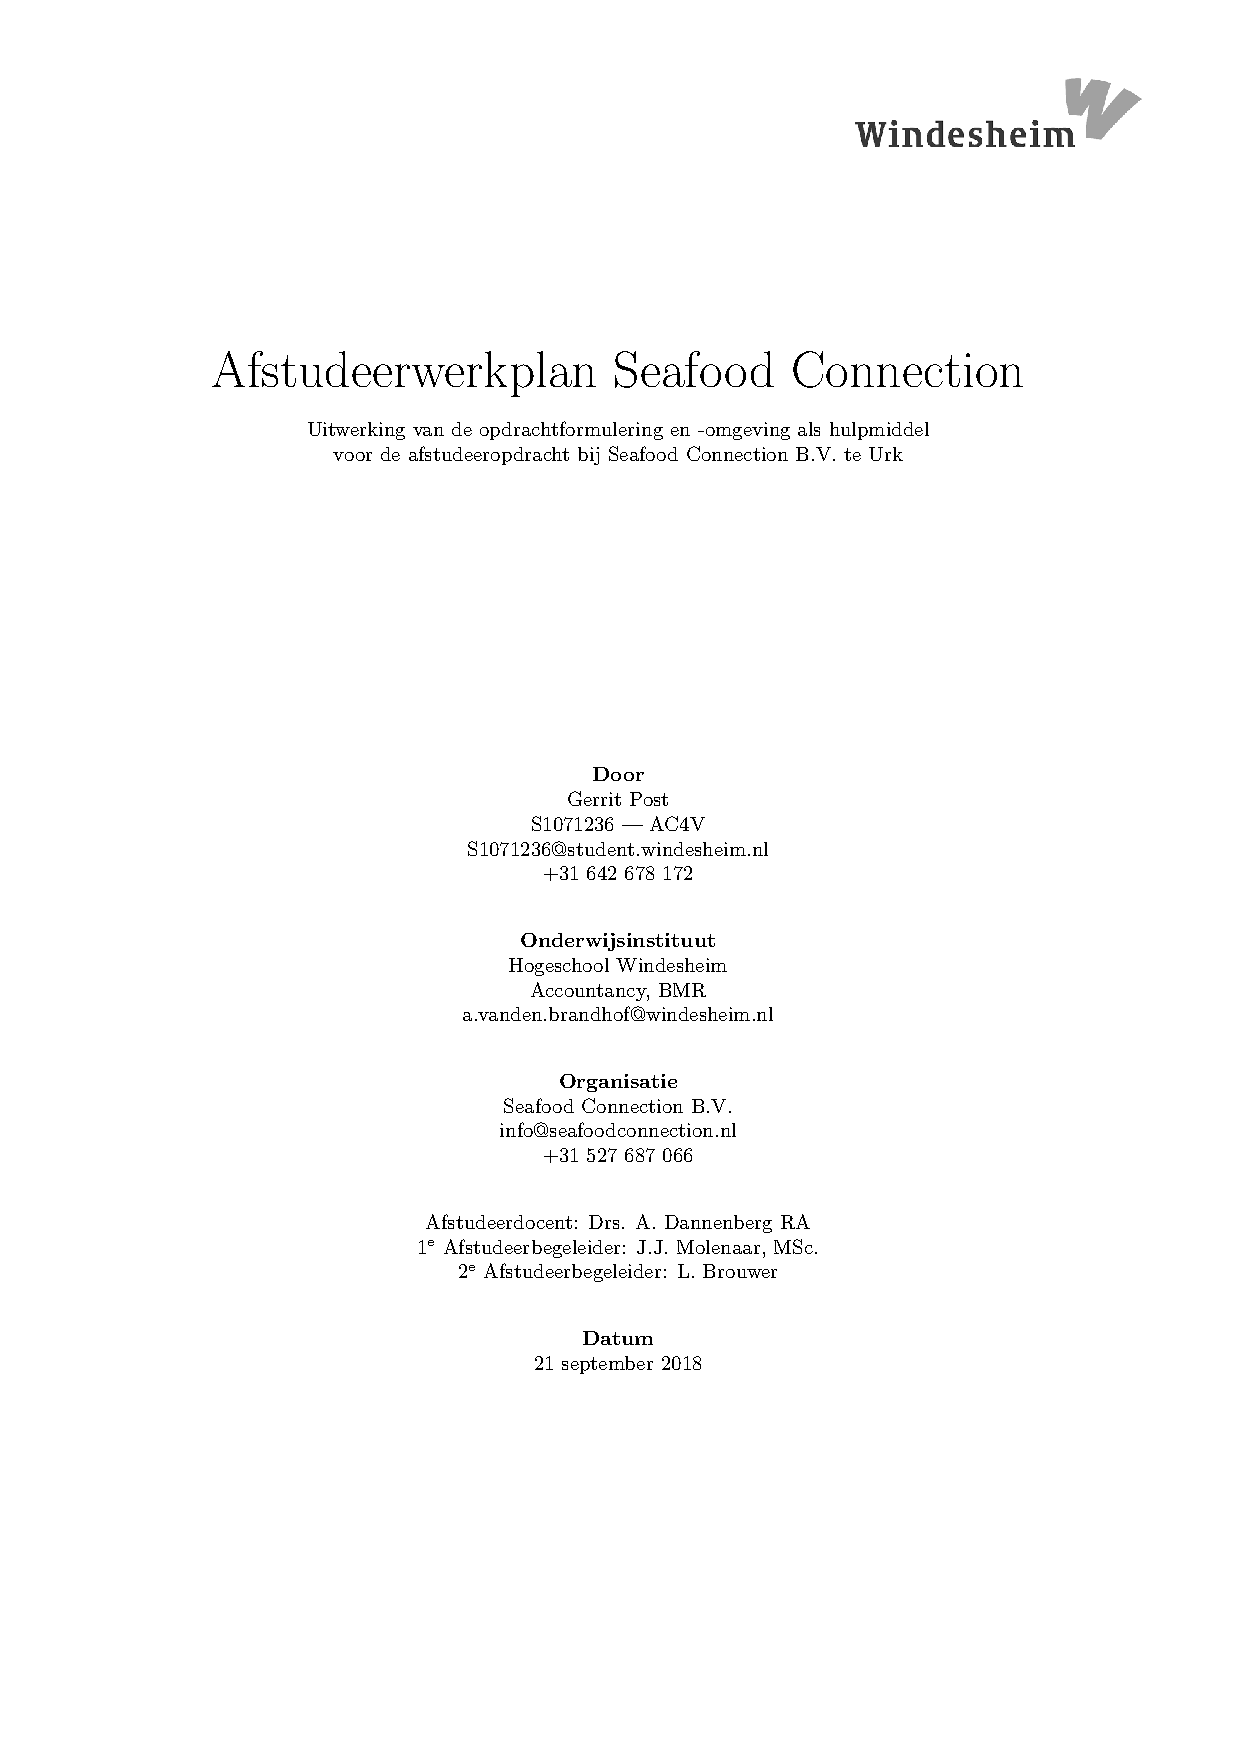
\includepdf{Titelpagina/titelpagina.pdf}
\afterpage{\blankpage}
\backgroundsetup{contents=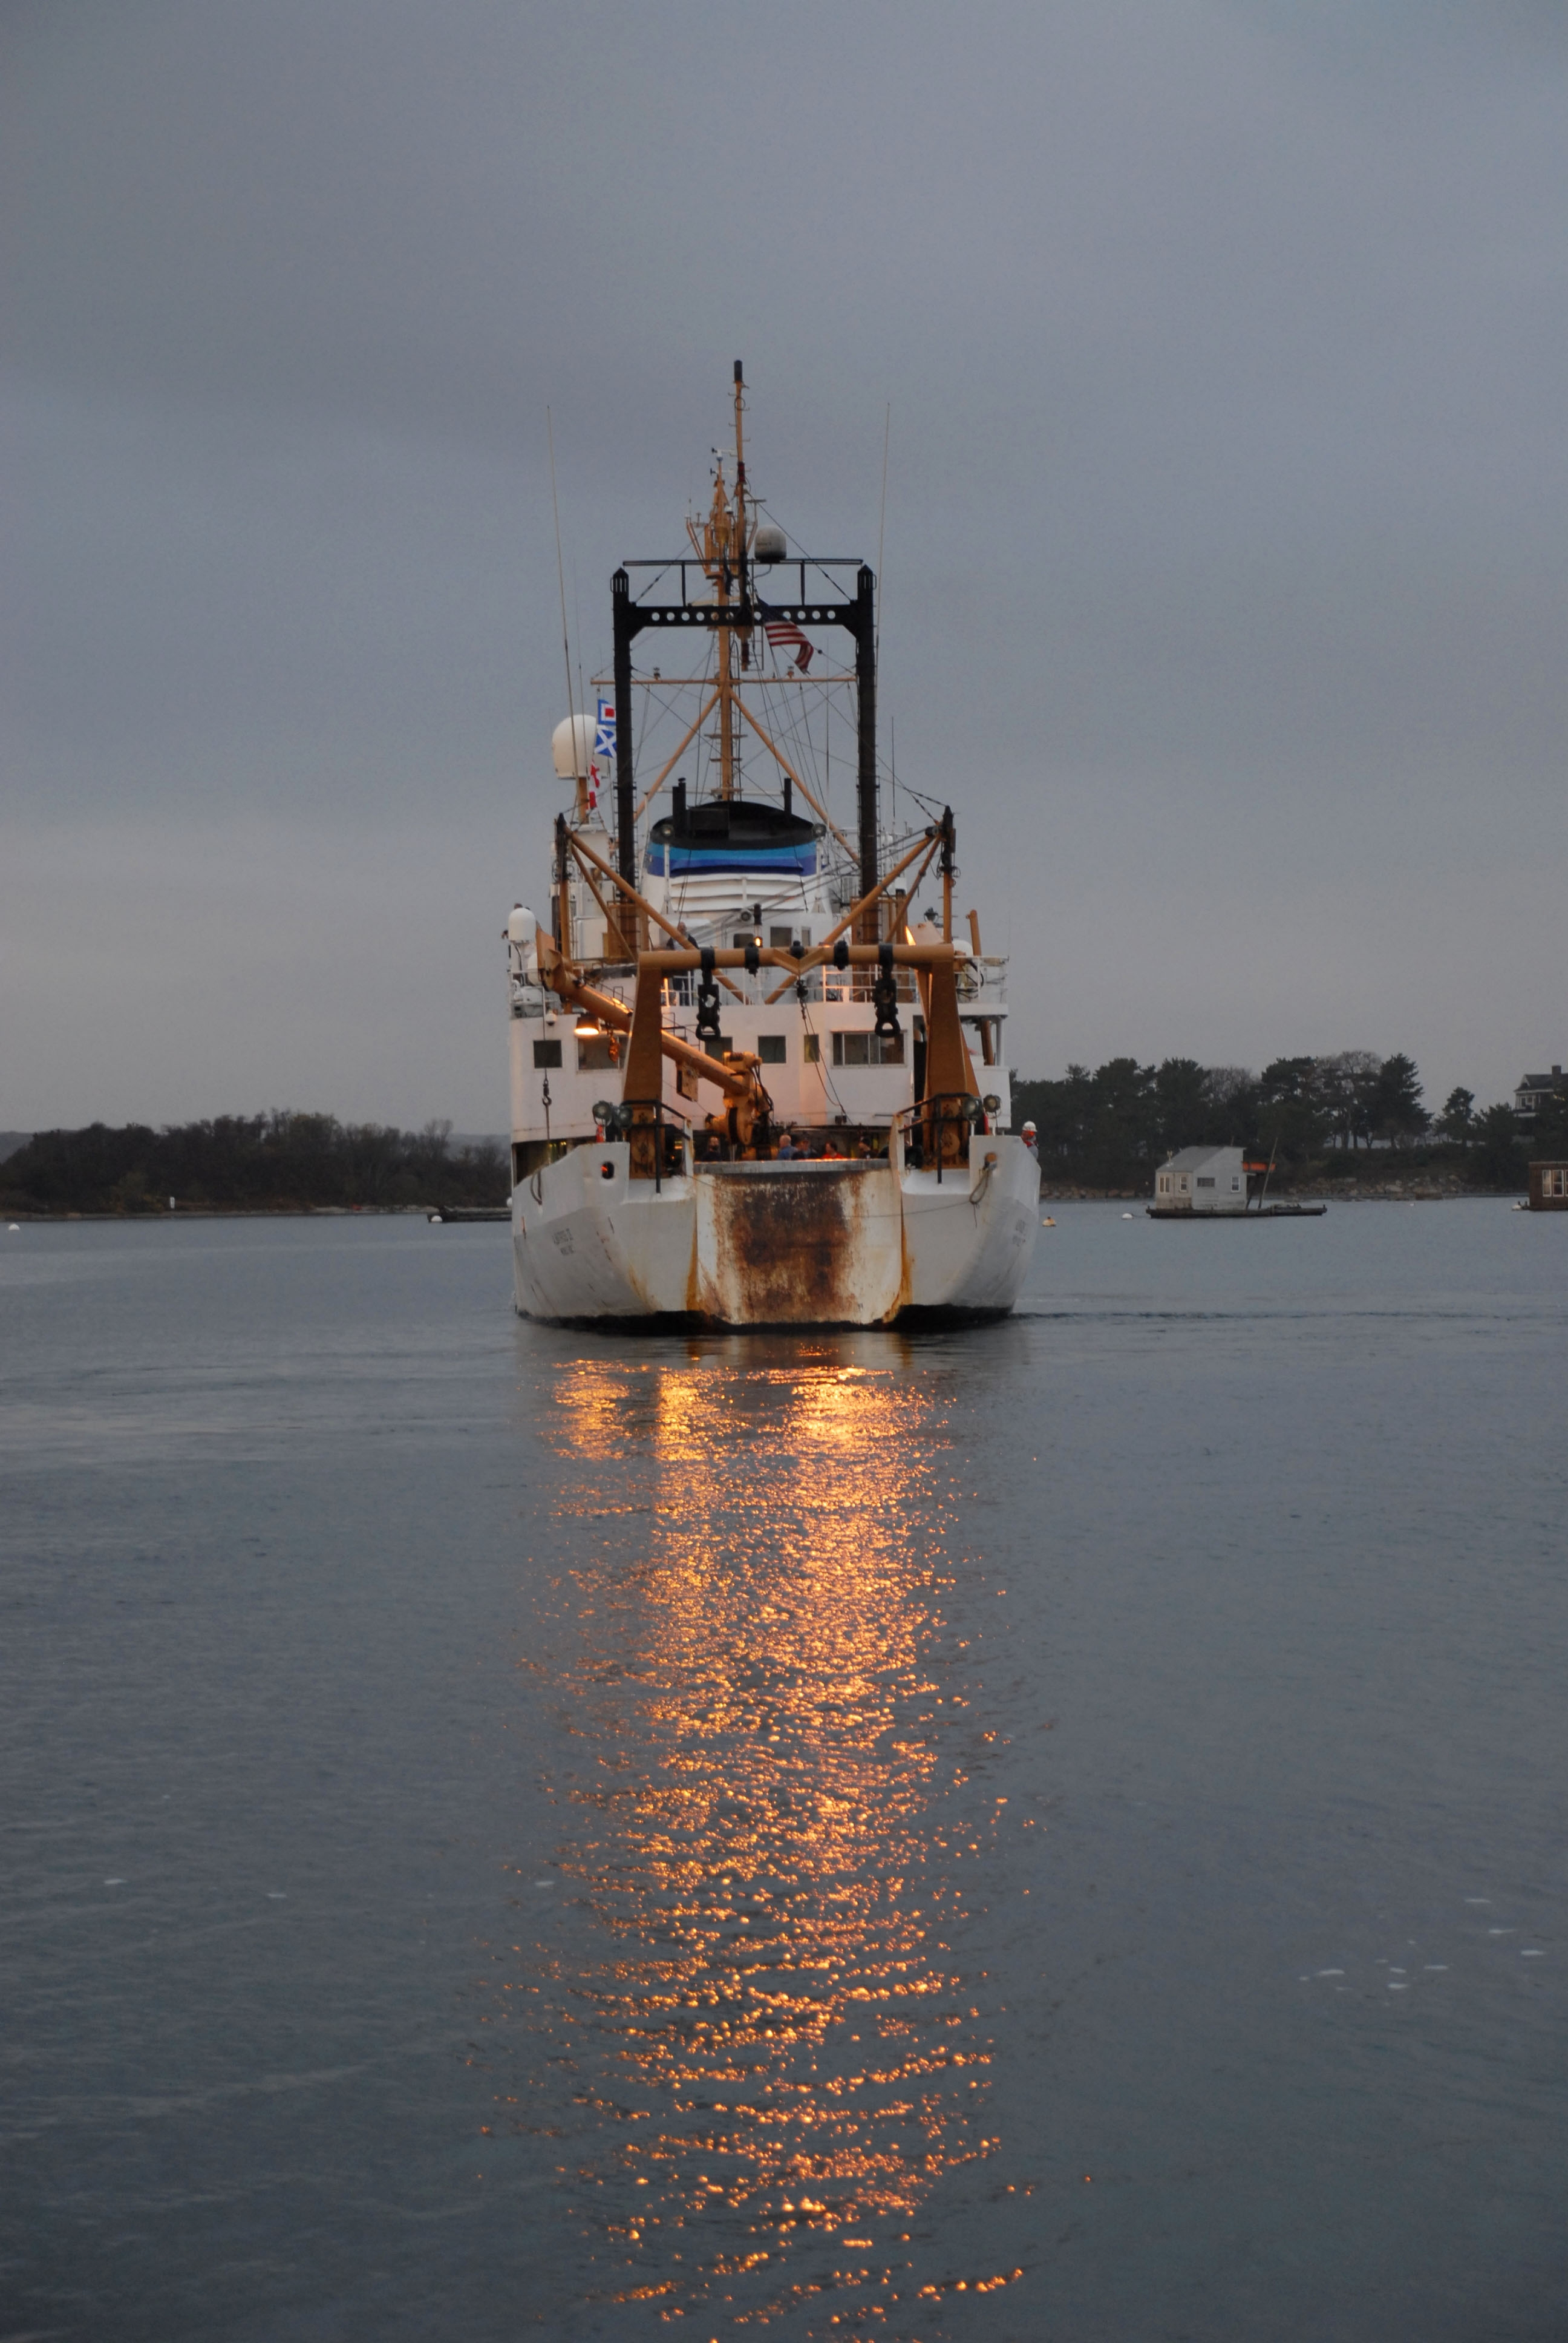
\includegraphics{3},angle=0,scale=1,opacity=1}
\BgThispage
%Titelblad wordt geïmporteerd als PDF want die is oneside en dit document twoside, zie eerste regel
%Na titelblad een lege pagina zodat er niets op de achterkant staat als hij dubbelzijdig wordt geprint

\chapter*{Voorwoord}
\thispagestyle{empty}
\backgroundsetup{contents=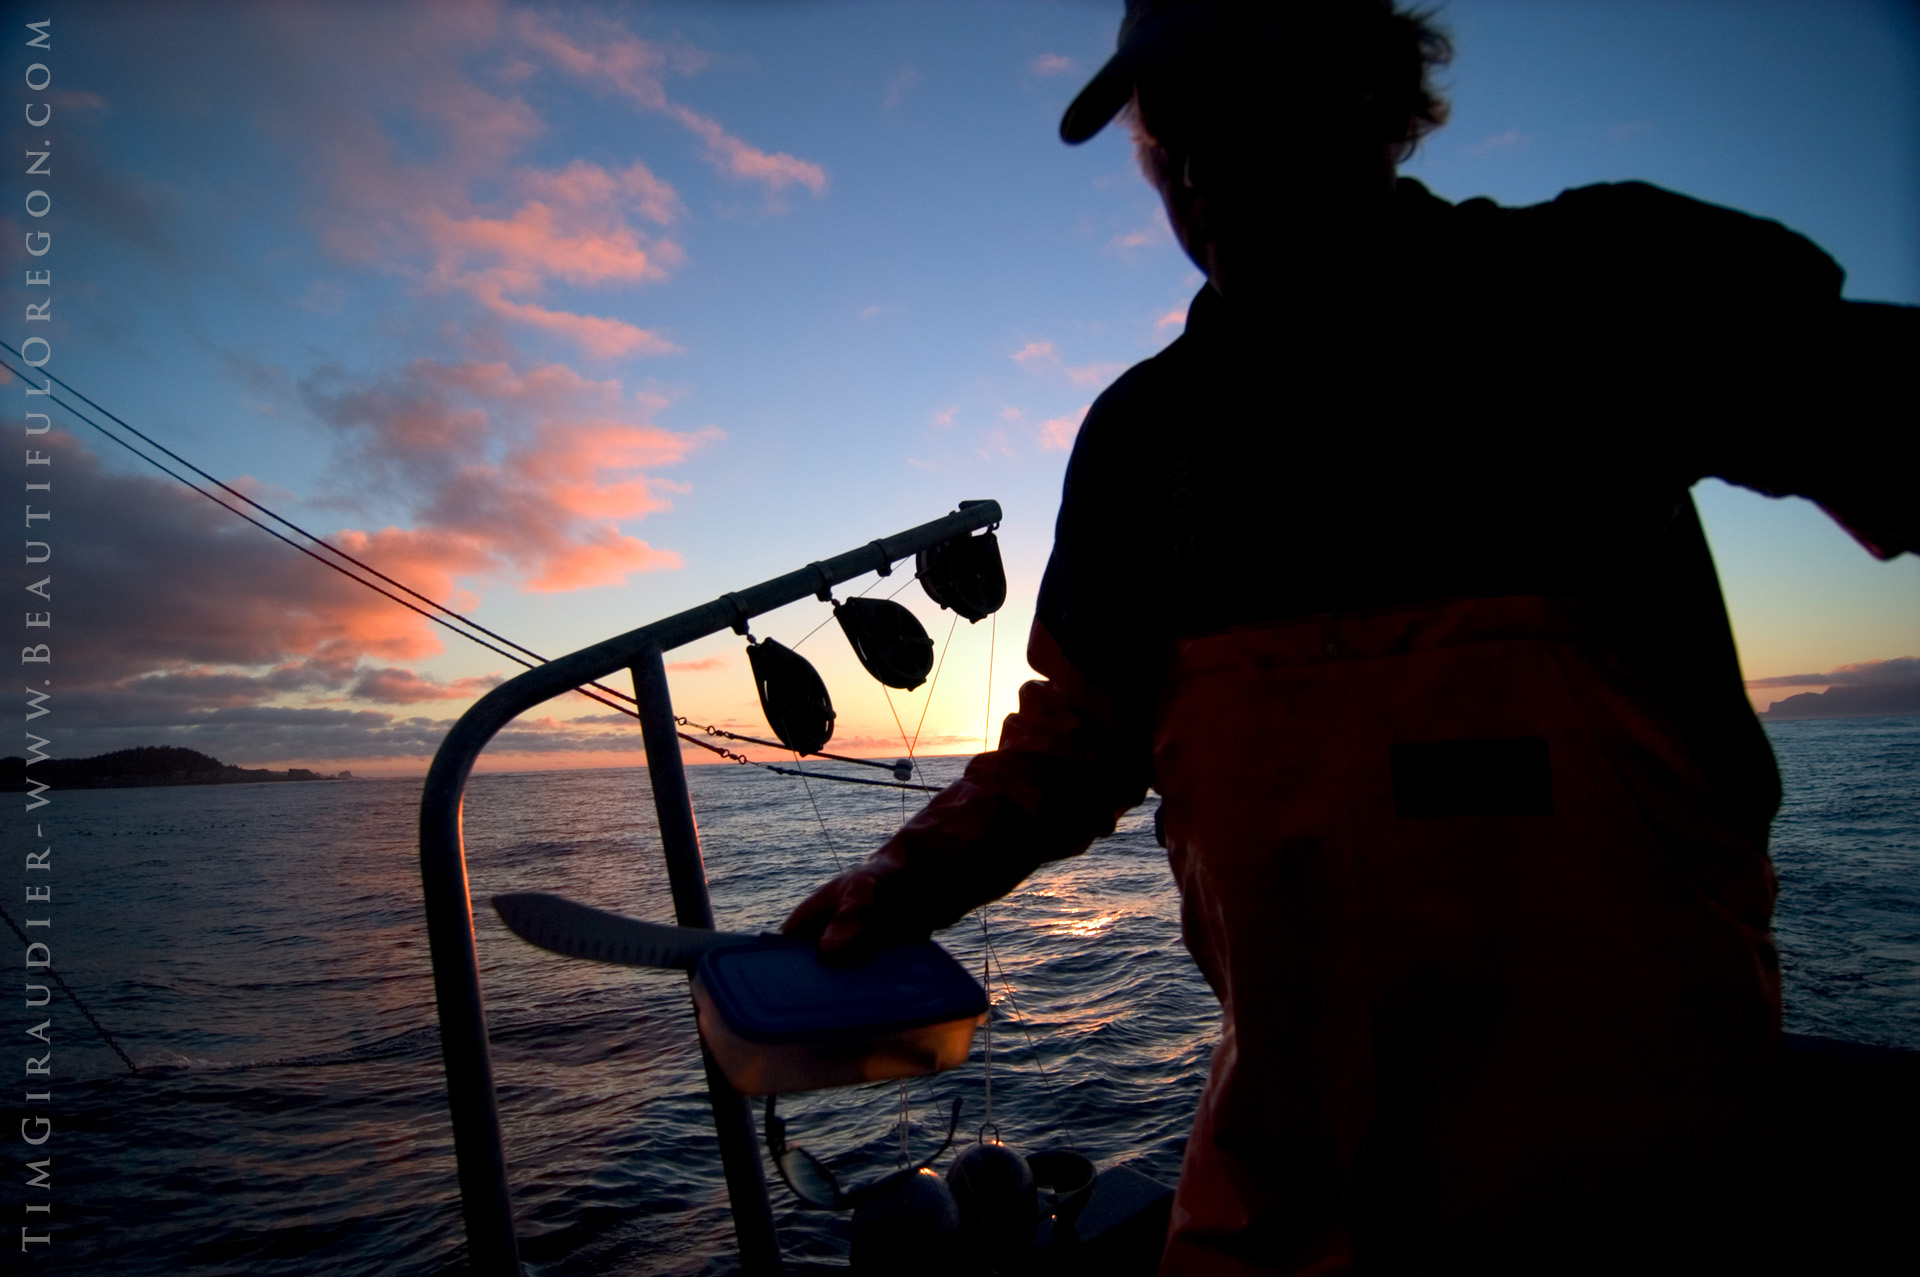
\includegraphics{7},angle=-2.5,scale=0.68,opacity=0.60,hshift=150}
\BgThispage
Het maken van een afstudeerproduct is een logische laatste stap na het succesvol afronden van het grootste gedeelte van de vakken voor mijn bacheloropleiding aan de Windesheim te Zwolle. Al voor de opdracht van start was gingen mijn handen kriebelen om deze afstudeerstage uit te kunnen voeren bij een uitdagende en atypische opdrachtgever. Dit verlangen was vooral gegrond in het feit dat ik een affiniteit voor AO/BIV aan het ontwikkelen was en graag wilde toetsen of mijn greep op dit vakgebied voldoende is. En waar beter deze kennis te toetsen dan bij een werkgever waar niet zomaar de geleerde typologieën gekopieerd en geplakt kunnen worden? \\
Mijn zoektocht begon naar een organisatie die in dit profiel past en graag met mij samen zou willen werken aan een nuttig eindproduct.

Eind juni kwam ik op de tennisbaan in gesprek met oud-collega Jurian, waar Seafood Connection ter sprake kwam als een interessante organisatie. Al snel zat ik aan tafel met Lucas Brouwer en voorgenoemde Jurian Molenaar waar Seafood Connection een steeds interessantere kandidaat leek te worden. Ik ben blij met de samenwerking die wij zijn aangegaan en ik hoop op een vruchtbare en productieve afstudeerperiode. Een bijzondere dank aan Rienk Bouma, Jon Bergsma, en Alidus Dannenberg voor de begeleiding vanuit school bij het formulerende proces van de opdracht. 

Ik wens de lezer veel plezier bij het lezen van dit afstudeerwerkplan en vanzelfsprekend ben ik bereid om vragen te beantwoorden en mee te nemen voor de opdracht. \\
\\
\textbf{Gerrit Post}\\
\textit{Student Accountancy, Hogeschool Windesheim}

%\vfill
%{\footnotesize\textsf{\textcolor{white}{Giraudier, Tim (2018). Cross Sound, Alaska.}}}

%Voorwoord met achtergrondafbeelding

%\chapter*{Samenvatting}
%\thispagestyle{empty}
%\lipsum[1-4]

\setcounter{page}{3} %Door importeren van PDF klopt paginanummer niet, hierbij gecorrigeerd
\tableofcontents
\thispagestyle{empty}


\chapter*{Inleiding}
\addcontentsline{toc}{chapter}{Inleiding} %Ongenummerde chapters komen niet in de ToC, met deze code wel
Ten behoeve van het definiëren en verkennen van de uit te voeren opdracht in het kader van het afstudeertraject, wordt in dit rapport met een brede blik gekeken naar de uitvoering hier van, waarbij er concreet uit wordt gewerkt welke zaken gaan spelen bij dit onderzoek. In samenwerking met de finance afdeling van Seafood Connection (hierna: SFC) wordt georiënteerd op de opdrachtformulering en wordt ook de opdrachtomgeving bekeken aan de hand van een bondige bedrijfsverkenning. 

Om de lezer een goed beeld te geven van de opdrachtomgeving wordt eerst bondig de bedrijfsachtergrond beschreven. Vervolgens wordt het de eerste stap van de onderzoekscyclus uitgewerkt volgens het model van Nel Verhoeven waar de probleemomschrijving breed en diep wordt uitgewerkt. In hoofdstuk drie wordt dit probleem omgezet in een concreet ontwerp waarin concreet wordt nagedacht over de invulling van de afstudeeropdracht- en periode. De competentieontwikkeling in hoofdstuk vier beschrijft de manier waarop de afstudeerstagiair gaat werken aan de landelijke en persoonlijke competentie- en ontwikkelpuntne. Als slot vindt u de bronnenlijst, bijlagen die verdiepend zijn voor dit plan en de tijdsplanning voor de afstudeerperiode. 


\chapter{Bedrijfsachtergrond}
\section{De onderneming}
\subsection{Omschrijving}
Opgericht in 1995, door huidig CEO J. (Jan) Kaptijn en C. (Chris) Goos met het innovatieve idee om een geselecteerd assortiment visproducten aan te bieden over de hele wereld zonder zelf ook maar een enkele visverwerkingsband te moeten aanschaffen. Seafood Connection werkt nauw samen met landen over de hele wereld om lokaal visproducten aan te kunnen bieden met een hoge kwaliteitsstandaard. Deze standaard wordt gegarandeerd door contacten van het bedrijf zelf grondige controles uit te laten voeren bij de leveranciers op locatie. Daarnaast wordt het productie- en verwerkingsproces gehouden aan hoge Europese standaarden als IFS, BRC, MSC en HACCP. \citep{sfcwebsite}

In 2013 werd de meerderheid van Seafood Connection gekocht door het Japanse Maruha Nichiro. Dit miljardenbedrijf, opgericht in 1880, is evenals SFC in alle uithoeken van de wereld te vinden. SFC hoopt met deze samenwerking te kunnen profiteren van de kennis en middelen van Maruha Nichiro, die naast de verkoop van visproducten het doel hebben om de hele waardeketen van de visindustrie te domineren. Dit betekent dat Maruha Nichiro een hand heeft in een groot aantal bedrijven dat rijkt van bedrijven in de aquacultuur, distributiecentrums en fabrieksschepen. Het moederbedrijf houdt het Nederlandse Seafood Connection nauwlettend in de gaten door expats, die hier op locatie zijn, aan procesoptimalisatie te laten werken en die rapportage doen aan het hoofdkantoor in Japan. \citep{sfcwebsite,Visserijnieuws}

\subsection{Fase}
Seafood Connection opereert in een markt die deels gedefinieerd wordt door prijsconcurrentie, het leveren van visproducten met kwaliteitskeurmerken is niet een nieuw fenomeen. Het onderscheidend karakter moet vaak ergens anders vandaan komen dan het voldoen aan minimum kwaliteitseisen. 

Het onderscheidend karakter is bij SFC bij een aantal zaken te merken. Ten eerste is er door de jaren heen zoveel kapitaal verworven dat SFC in een bevoorrechte positie is waar zij op grote schaal kan inkopen. Tevens heeft SFC een select aantal leveranciers die nauwkeurig gekozen zijn op hun bereidbaarheid om vis te leveren die aan de normen SFC voldoen. SFC opereert dus in een verzadigde markt, maar groeit altoos door haar onderhandelingspositie.

\subsection{De activiteiten in perspectief} \label{beschr:activiteiten}
Om een volledig beeld te krijgen van de ondernemingsactiviteiten is het belangrijk om aandacht te besteden aan de financiële kant van de onderneming. Hier gebeurt namelijk iets opmerkelijks, wanneer bijvoorbeeld de financiële ratio's vergeleken worden met algemeen geaccepteerde normen valt Seafood Connection op het eerste blik buiten de boot. Om deze ratio’s te beoordelen moeten zij eerst in context worden geplaatst, deze kunnen niet één-op-één vergeleken worden met normen die worden gehanteerd voor een regulier handelsbedrijf. Het is voor een bedrijf als SFC namelijk aantrekkelijk om relatief veel schulden op zich te nemen ten opzichte van haar bezittingen. SFC koopt grootschalig in voor verscheidene producten op een groot aantal markten. Dit betekent dat wanneer een grote batch visproducten wordt gekocht, het gebruikelijk is dat levering pas na één maand plaatsvindt. Na levering blijft de voorraad doorgaans twee maanden op voorraad voor het verkocht wordt, waarbij betaling van deze order één tot twee maanden na de aflevering van deze goederen plaatsvindt. In feite ontvangt Seafood Connection vaak pas na vier tot zes maanden na investering pas haar geld terug. De ratio’s die hiermee verbonden zijn kunnen dus niet ontkoppeld worden aan de inherente eigenschappen van bulkinkoop op een internationale markt. \citep{jaarrapport2017}

\begin{table}[h]
    \centering
    \caption{Kengetallen jaarrekening over 2017 \citep{jaarrapport2017}}
    \begin{tabular}{l r r}
        \toprule
        \textbf{Kengetal} & \textbf{Ultimo 2017} & \textbf{Ultimo 2016} \\
        \midrule
        Rendament TV & 5,6\% & 4,9\% \\
        Solvabiliteit & 24,6\% & 20,8\% \\
        Liquiditeit & 55,4\% & 52,9\% \\
        \bottomrule
    \end{tabular}
    \label{tab:kengetallen}
\end{table}

Uit het jaarrapport over 2017 worden de financiële ratio’s uit tabel \ref{tab:kengetallen} ontleend. Deze cijfers gelden voor de peildatum van respectievelijk 31 december 2017 en 2016.

Het rendement op het totale vermogen is berekend als ((nettowinst + betaalde rente) / balanstotaal), de solvabiliteit als (eigen vermogen / totaal vermogen), en de liquiditeit als (vlottende bezittingen / kortlopende schulden). \citep{jaarrapport2017}

\newpage
\section{De organisatie}
organisatie is veranderd van lagen naar groepen (geografisch, per product, en markt), verdubbeling personeel, nieuw product sushi

\subsection{Typering}
Seafood Connection is een handelsbedrijf in diverse diepvries visproducten met daarnaast in beperkte mate doorstroom van eigen goederen met een eenvoudig, technisch omzettingsproces \citep{aoibsfc}. Voor de verschillende bedrijfsactiviteiten fungeert Seafood Connection als:

\begin{enumerate}
    \item Handelsbedrijf dat hoofdzakelijk aan andere bedrijven levert
    \item Productiebedrijf met homogene massaproductie
    \item In zeer beperkte mate dienstverlening aan derden (door commissie op verkopen aan derden)
\end{enumerate}

Volgens de modellen van Starreveld is SFC een \textit{Handelsbedrijf op rekening}. Belangrijke aanknopingspunten voor de interne controle zijn de geautoriseerde brutomarge en prijsprocedure; de harde functiescheiding tussen de afdelingen: inkoop, opslag, verkoop en administratie; én de inventarisatie als het sluitstuk van de geld-goederenbeweging. In de grotendeels zelf-gerapporteerde quick scan geeft SFC zelf aan dat procedures verankerd in het systeem liggen, maar tegelijkertijd flexibel zijn voor optimalisatie; er is een sterke functiescheiding tussen inkoop, opslag en administratie. Echter geeft zij zelf aan dat er sprake is van een open magazijn, dat niet alléén beheerd wordt door de magazijnmeester, het magazijn wordt door verschillende mensen geïnventariseerd, en er is sóms onafhankelijke controle van de verkoopprijzen. \citep{bivperspectief,quickscan}

Een ander belangrijk detail voor de Administratieve Organisatie is dat het bedrijf in sterke mate gebruik maakt van automatisering. Zo is er een bevoegdheidsmatrix waarin beschikkende medewerkers geautoriseerd of geblokkeerd zijn om bepaalde handelingen uit te voeren. Daarnaast zijn er limieten voor bepaalde handelingen als de hoeveelheid in te kopen vreemde valuta. In de quick scan geeft de organisatie weer dat (bijna) altijd gebruik wordt gemaakt van automatisering. \citep{quickscan}

\subsection{Inrichting}
Seafood Connection is vijftig gemotiveerde werknemers sterk. Het kantoor op Urk vervult alle bedrijfsfuncties op één locatie. De organisatie heeft vier niveaus: het managementteam (MT) dat de strategie formuleert, de unitmanagers (UM) die hun afdelingen aansturen, managers die het aanspreekpunt zijn voor hun deelprocessen in de verschillende afdelingen, én assistants die de afdelingen ondersteunen met verschillende werkzaamheden. SFC is een lijn-staforganisatie met een gedeelde P-, G-, en M-indeling opgedeeld in de afdelingen: inkoop, opslag, verkoop, finance, ICT and productie, HRM, compliance, en marketing verdeeld over vier segmenten: wholesale, retail, industry, en group (geografisch beheer). \citep{quickscan}

\section{De branche}
Kenmerken voor succes in de branche zijn ogenschijnlijk het hebben van een affiniteit voor duurzaamheid, naleving van kwaliteitsstandaarden en goed toegankelijk zijn zodat verse vis in elk jaargetijde geleverd kan worden. In mindere mate is er ook sprake van prijsconcurrentie, maar dit is vooral te merken bij de verkoop van diepvriesvis en niet zozeer bij verse filet. 

Seafood Connection is niet de enige aanbieder van vis. SFC opereert op Urk, één van de grootste centrums voor de visverwerking in Nederland, de CFO van Seafood Connection zegt hier zelf over dat het een gezonde hoeveelheid concurrentie voor de kiezen heeft. Het is dan ook niet verrassend dat de onderneming als grootste succescriteria heeft gekozen om te winnen in de markt, dit plaatst zij boven criteria als het beschikken over een zo uniek en nieuw mogelijk productassortiment of efficiënte bedrijfsvoering. 

De missie van Seafood Connection is om het volgende te anticiperen: klantbelangen, de behoefte aan duurzame visproducten, en nieuwe trends. De onderneming wil dit realiseren door nieuwe partners te verkrijgen in cruciale markten in Europa, Amerika en Azië. Tevens worden nieuwe keteninnovaties verkregen door fusies en overnames in de visindustrie. \citep{sfcwebsite} \\
\\
\color{red}
Indien relevant ook nog: Gevolgde strategie, concurrentie, marktfactoren, belangrijke regelgeving. Oordeel van de accountant
\color{black}

\chapter{Probleemanalyse}
\section{De aanleiding}
\subsection{Aanleiding en probleemomschrijving}
De AOIB bij Seafood Connection is in lichte mate verouderd, concreet betekent dit dat sinds de laatste update er nieuwe afdelingen zijn ontstaan, er nieuwe functies zijn gecreëerd of zijn veranderd, en dat het organogram veranderd is. Het bedrijf is sinds de laatste update haast verdubbeld qua omzet en personeel. Een update is dus hoognodig om te voorkomen dat de vastgelegde AOIB niet overeenkomt met de werkelijkheid. Wanneer de vastgelegde AO niet overeenkomt met de werkelijkheid zal dit tot gevolg hebben dat er geen fundament is voor de interne beheersing van de bedrijfsvoering. \citep{bivpraktijk}

Juist door deze licht verouderde AO is er een discrepantie tussen de daadwerkelijke bedrijfsprocessen en de formele vastlegging hiervan. Het grootste bedoelde knelpunt hier is de vastlegging van de organisatorische maatregelen rond de financiële geldstromen. Zoals eerder beschreven in paragraaf \ref{beschr:activiteiten}, haalt Seafood Connection haar bestaansgrond uit het feit dat er op grote schaal wordt ingekocht en verkocht op een internationale markt. De geldgoederenstroom is een cruciaal deel van de bedrijfsvoering die op het moment niet uitgebreid en doordacht is vastgelegd. \citep{aoibsfc}

is er nog niet een beleid omtrent de \textit{treasury}. Treasurybeleid is de manier waarop een onderneming haar \textit{treasures} (of ook: schatten) beheert. De praktische invulling van het treaurybeleid wordt omschreven in het door het management opgestelde treasury statuut. 
Deze statuut is \textbf{intern} gericht door in kaart te brengen hoe de verschillende processen rond de financiële beheersing horen te functioneren, er wordt bijvoorbeeld dus beschreven wie welke functie heeft in het geldgoederenproces en welke controles daarop uitgevoerd worden. \\
Ook is de statuut \textbf{extern} gericht aan stakeholders door de verantwoording die wordt afgelegd, door het management, over het geldbeheer. \citep{handreiking} \\
In deze en volgende rapportage wordt de volgende definitie gehanteerd voor de term treasury statuut: 

\begin{displayquote}
Het treasury statuut is een door het management opgesteld rapport waarin de bevoegdheden, verantwoordelijkheden, toezichtmaatregelen, de sturing, en beheersing geformuleerd worden ten aanzien van financiële vermogenswaarden, financiële geldstromen, financiële posities en de hieraan verbonden risico’s. \\
\citep{ede,handreiking} \label{def:treasury}
\end{displayquote}
\noindent
Zie ook \hyperlink{bij:treasury}{bijlage 1} voor een overzichtelijke uitwerking van het begrip treasury statuut.

Samenvattend worden de huidige bestaande organisatorische maatregelen en processen in kaart gebracht. Daarnaast is het management van SFC bewust dat er op een navolgbare en verantwoordelijke manier omgegaan moet worden met financiële middelen; immers handelt het bedrijf met een uitputbare hoeveelheid vreemde valuta en is er een hoge mate van liquiditeit vereist om het bestaan van het bedrijf in de toekomst te kunnen garanderen.

\subsection{Betrokken partijen}
De betrokken partijen bij dit probleem zijn echter niet alleen de leden van het management. De inrichting en het vormgeven van de organisatie heeft direct invloed op alle bedrijfsprocessen en de werknemers werkzaam in de waardeketen. Het is voor de beheersing van de processen belangrijk dat de afstudeerstagiair gesprekken aangaat met niet alleen de afdelingshoofden, maar ook de assistenten die direct onder leiding van het middenmanagement staan. Bij de dagelijkse werkzaamheden wordt niet bewust nagedacht over de administratieve maatregelen die voor SFC gelden, om deze reden is onderzoek noodzakelijk om onder andere te kijken of er in de praktijk de al dan niet aanwezige functiescheiding wordt nagevolgd. Sturend in het onderzoek is het management en de CFO die de informatieverstrekkers zijn en de uiteindelijke afnemer zullen zijn van het eindproduct. 

Een aantal partijen zijn niet (volledig) betrokken bij het afstudeerproduct. Ten eerste is de primaire accountant van SFC niet deel van de belangendriehoek (de stagiair, de opdrachtgever, de opleidingsinstantie). Deze keuze is bewust door het managent gemaakt omdat de AOIB intern gericht is en de treasury statuut een aflegging van de verantwoording is vanuit het management. 
Ook de deelnemingen, groepsmaatschappijen, joint ventures, en andere verbonden onderneming zijn niet deel van het onderzoek. Het productverslag is enkel de interne beheersing van Seafood Connection.

\subsection{Ontstaan opdracht}
Deze opdracht is ontstaan vanuit de finance afdeling in het afgelopen jaar. Deze handelt registrerend en controlerend ten behoeve van de geld-goederenstroom. De intern beschikkende afdelingen – inkoop en verkoop – werken nauw samen met finance voor de bewaking en afdekking van valuta- en koersrisico. Het management en de afdeling finance hebben samen een voorkeur voor een formeel vastgelegd beleid en zochten hiervoor een passende afstudeerder. Daarnaast was de licht verouderde AOIB toe aan vernieuwing.

Het enige voorwerk dat voor deze opdracht is verricht is het opstellen van de bestaande AOIB jaren terug en het opzetten van de geautomatiseerde systemen voor het inkopen van vreemde valuta.

\section{De doelstelling}
Het eerste onderdeel van de probleemomschrijving bevat het formuleren van de doelstelling. Bij de doelstelling geef je aan wat de opdrachtgever met het onderzoek wil bereiken (het omvat de doelen en wensen van de opdrachtgever).

\section{Probleemomschrijving}
Vervolgens formuleer je de probleemstelling. De probleemstelling wordt geformuleerd als een vraag! De probleemstelling wordt ook wel centrale vraagstelling genoemd. Kenmerkend is dat deze vraag gaat over een bepaalde periode (1) en dat de vraag alle belangrijke begrippen bevat.
(2). De probleemstelling moet verder samenhangen met de doelstelling. Het is belangrijk om hierbij al rekening te houden met het vraagtype9. Het vraagtype bepaalt namelijk welke onderzoeksmethode nodig zal zijn. Tenslotte zal de hoofdvraag worden uitgesplitst in afgebakende deelvragen. Met behulp van de deelvragen ga je de kernbegrippen uit de hoofdvraag nader onderzoeken. Een goed middel om de deelvragen te formuleren is gebruik te maken van een boomdiagram10.

\subsection{Relevante aspecten}
Belangrijk om in gedachten te houden bij deze opdracht is dat deze opdracht zowel intern als extern is gericht. Intern wordt verslag gedaan over de administratieve organisatie en deze wordt geüpdatet. Het is dus niet de bedoeling dat derden dit document voor handen krijgen. Het op te stellen treasury statuut is echter wel bedoeld voor derden want het is een verantwoording van het management over hoe er wordt omgegaan met financiële middelen. Stakeholders kunnen met dit document een verhelderende blik in de onderneming krijgen. Bij de uitwerking van deze twee deelproducten moet de bedoelde doelgroep wel in het oog worden gehouden.

\section{Begripsafbakening}
Het derde onderdeel van de probleemanalyse omvat de begripsafbakening. Hierbij geef je duidelijk aan wat jij verstaat onder de begrippen die voorkomen in hoofd- en deelvragen. We noemen dit het operationaliseren van de begrippen.

\section{Theoretische ondersteuning}
Bij het onderdeel theoretische ondersteuning zoek je meerdere bronnen voor een theorie of model dat je wilt of gaat gebruiken in je onderzoek. Geef hierbij een duidelijke argumentatie welke bron de voorkeur geniet.

\chapter{Onderzoeksontwerp (fase 2 onderzoekscyclus)}

\chapter{Competentieontwikkeling}

\printbibliography
\addcontentsline{toc}{chapter}{Bibliografie}

\chapter*{Bijlagen}
\addcontentsline{toc}{chapter}{Bijlagen}
\section*{\hypertarget{bij:treasury}{Bijlage 1}: het treasury statuut}
\addcontentsline{toc}{section}{Bijlage 1: het treasury statuut}
\begin{figure}[ht]
    \centering
    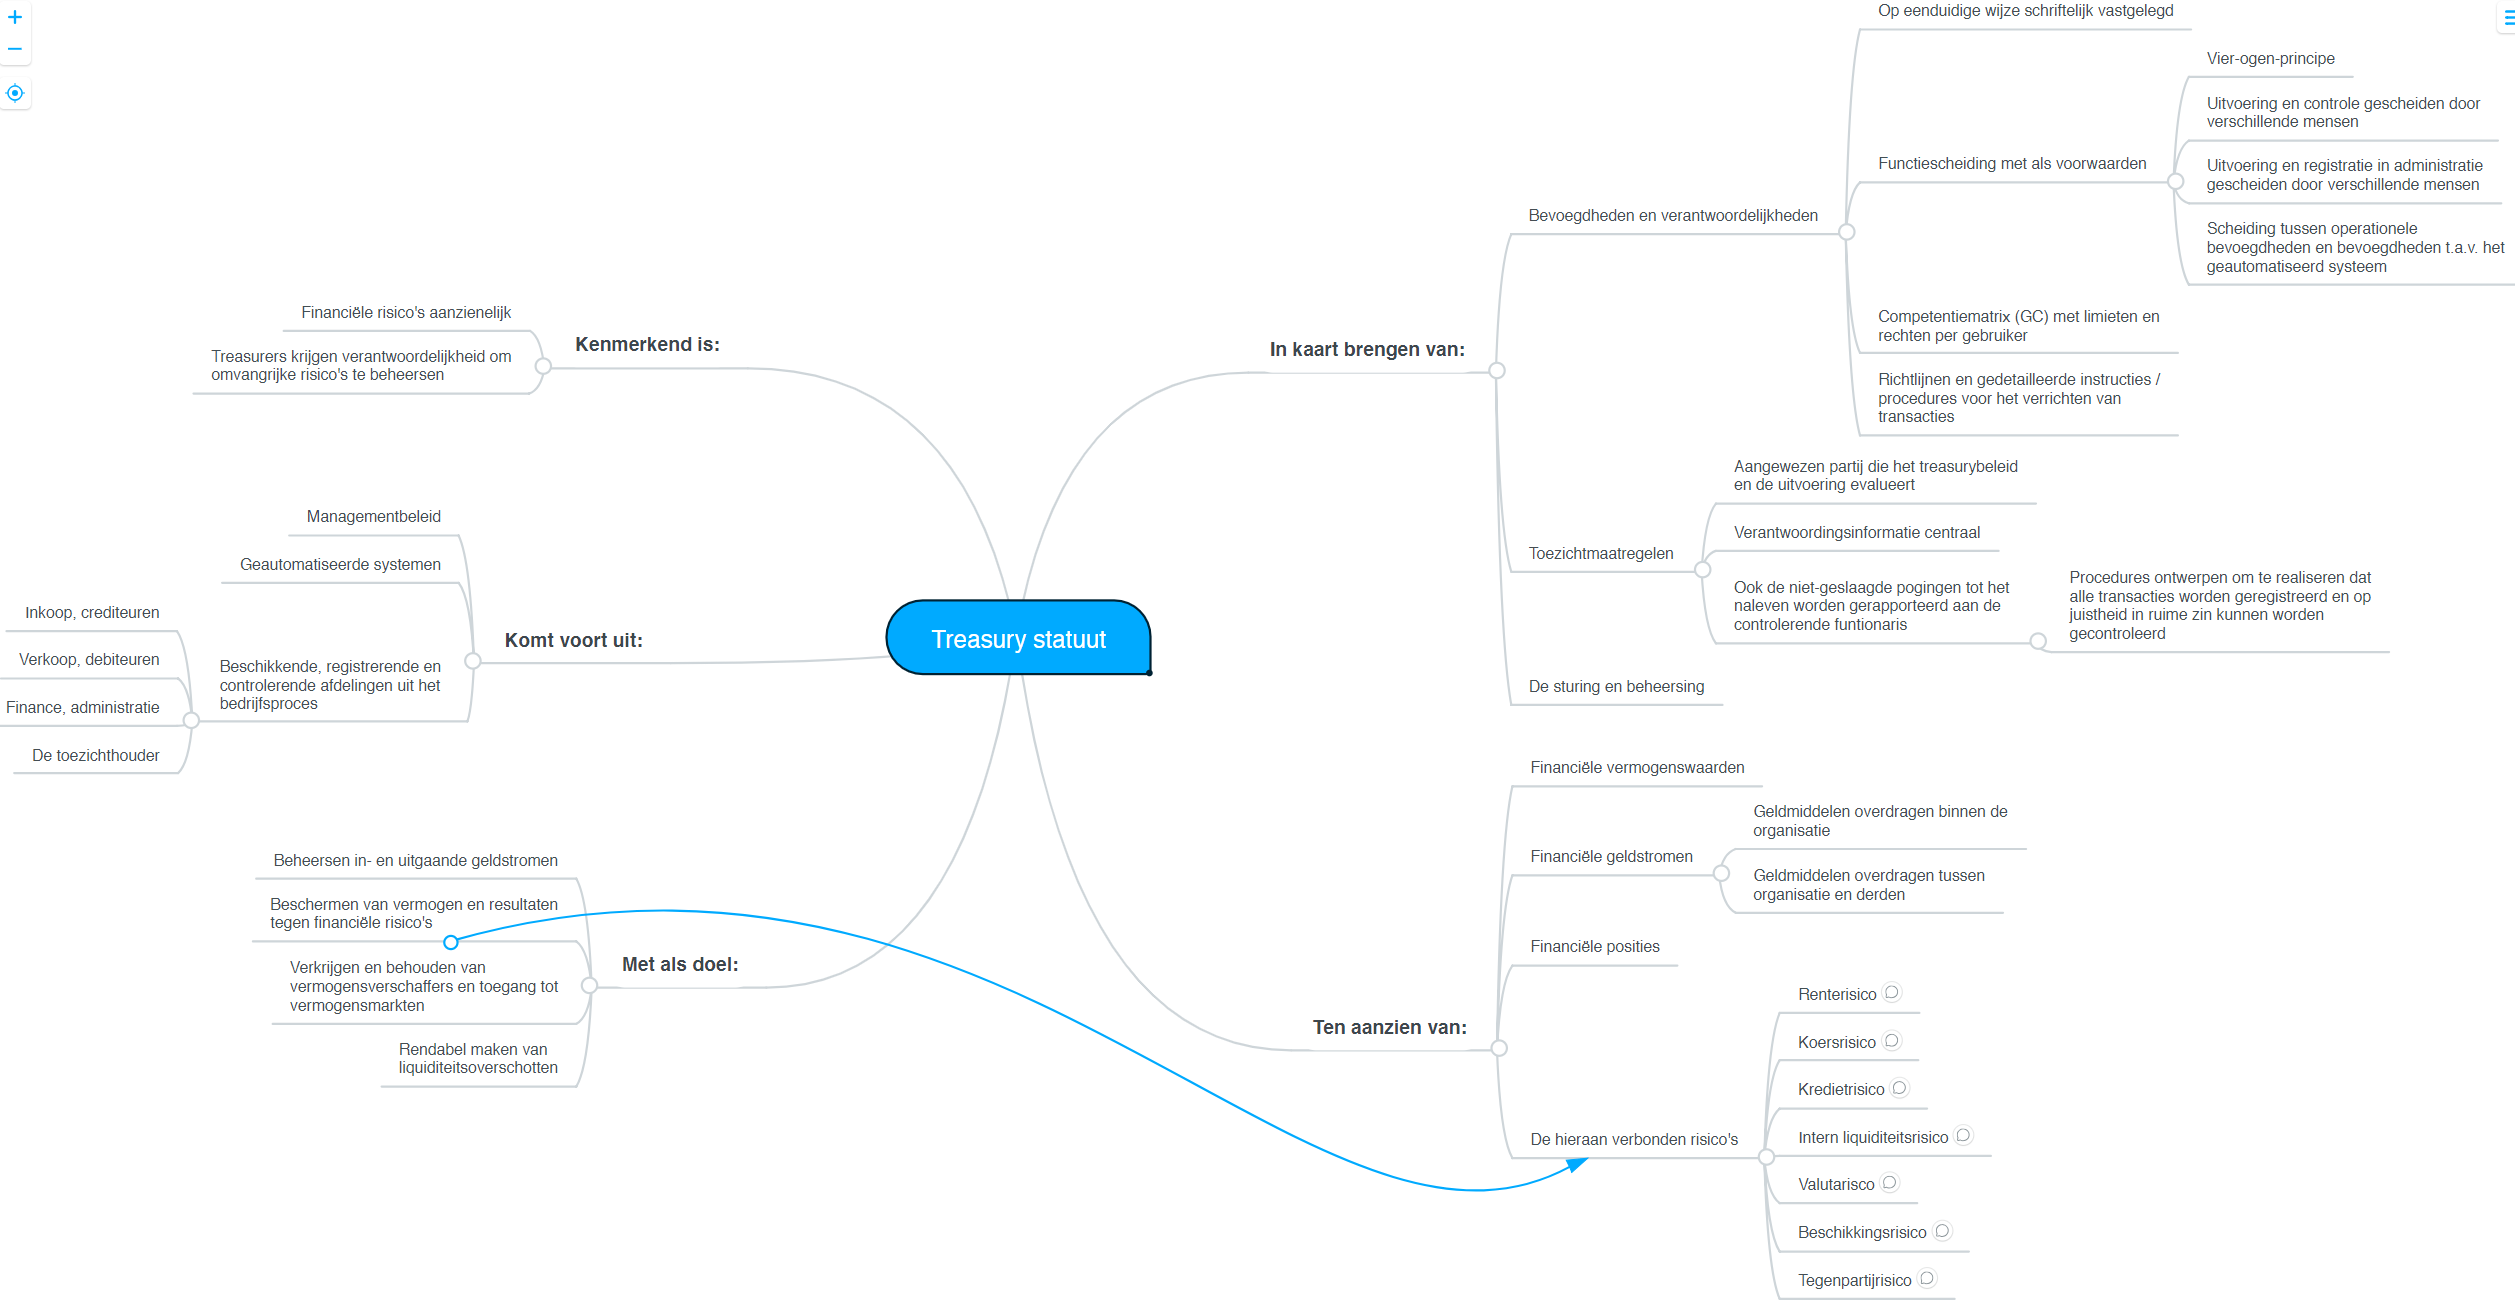
\includegraphics[angle=90,height=0.70\textheight]{treasury}
    \label{fig:mmtreasury}
\end{figure}

\chapter{Tijdsplanning en communicatie}

\end{document}